\sectioncounter{4}
  \section{函数的单调性和奇偶性}

  \subsection{知识梳理}
  函数的\myindex{单调性} (monotonicity) 描述的是其图象的变化趋势. 当沿 $x$~轴正向看时, 若图象上升, 则称函数单调递增加 (单增);
  若图象下降, 则称函数单调递减少 (单减). 设函数为 $f(x)$, 且 $x_1<x_2$, 则
  \[f(x_1)<f(x_2)\Leftrightarrow f(x)\nearrow;\quad
    f(x_1)>f(x_2)\Leftrightarrow f(x)\searrow.\]
  若只设 $x_1\neq x_2$, 则
  \begin{align*}
    &\frac{f(x_1)-f(x_2)}{x_1-x_2}>0\Leftrightarrow
     (f(x_1)-f(x_2))(x_1-x_2)>0\Leftrightarrow
     f(x)\nearrow;\\
    &\frac{f(x_1)-f(x_2)}{x_1-x_2}<0\Leftrightarrow
     (f(x_1)-f(x_2))(x_1-x_2)<0\Leftrightarrow
     f(x)\searrow.
  \end{align*}
  常见函数的单调性的决定因素如下: 
  
  $f(x)=kx+b$: $k>0$ 时 $\searrow$, $k<0$ 时 $\nearrow$;
  
  $f(x)=\frac{k}x$: $k>0$ 时分段 $\searrow$, $k<0$ 时分段 $\nearrow$;
  
  $f(x)=ax^2+bx+c$: $a$ 决定抛物线开口方向, $-\frac{b}{2a}$ 决定对称轴位置;
  
  $f(x)=a^x$, $g(x)=\log_a x$: $0<a<1$ 时 $\searrow$, $a>1$ 时 $\nearrow$.
    
  函数的\myindex{奇偶性} (odevity) 描述的是其图象的对称性. 
  \mymarginpar{一般地, 设函数 $f(x)$ 的定义域为 $\mathbb{R}$, 则\\
    \hbox{\quad} $f(x)$ 关于直线 $x=a$ 对称 \\
     $\Leftrightarrow f(a+x)=f(a-x)$\\
     $\Leftrightarrow f(x)=f(2a-x)$;\\
    \hbox{\quad} $f(x)$ 关于点 $(a,b)$ 对称\\
     $\Leftrightarrow f(a+x)+f(a-x)=2b$.}
  若图象关于 $y$~轴对称, 则称其为\myemph{偶函数};
  若图象关于原点对称, 则称其为\myemph{奇函数}. 设函数为 $f(x)$, 则
  \begin{align*}
    &f(x)\text{\,为偶函数}\Leftrightarrow f(-x)=f(x)\Leftrightarrow f(-x)-f(x)=0;\\
    &f(x)\text{\,为奇函数}\Leftrightarrow f(-x)=-f(x)\Leftrightarrow f(-x)+f(x)=0.
  \end{align*}
  由定义可以知道, 
  
  (1) 判断函数奇偶性之前, 应确保其定义域关于原点对称;
  
  (2) 函数按奇偶性可分为: 奇函数, 偶函数, 既奇又偶函数 (可以认为只有一个), 非奇非偶函数;
  
  (3) 若 $0$ 在奇函数 $f(x)$ 的定义域中, 则必有 $f(0)=0$ (并非充要条件);
  
  (4) $f(x)$ 为偶函数 $\Leftrightarrow$ $f(x)$, $f(|x|)$, $f(-x)$ 中有两者相等.

  \lianxi
  \begin{exercise}
    函数 $f(x)= x^2-2x$ 的单调递增区间为\,?
  \end{exercise}
  
  \beginsolution
    对称轴 $x=1$, 单调递增区间为 $[1,+\infty)$.
  \endsolution
  
  \begin{exercise}
    若 $f(x)$ 是定义在 $[-1,1]$ 上的单调递增函数, 
    且 $f(x-1)<f(1-3x)$, 求 $x$ 的取值范围.
  \end{exercise}
  
  \beginsolution
    由题 $-1\leqslant x-1<1-3x\leqslant 1$, 解得 $x\in\Big[0,\frac12\Big)$.
    
    \varexercise 若 $f(x)=x^3+x$, 解不等式 $f(x-1)<f(1-3x)$.
    
    因为 $f(x)$ 在 $\mathbb{R}$ 上单调递增, 所以 $x-1<1-3x$ 即 $x\in\Bigl(-\infty,\frac12\Bigr)$.
    
    \varexercise 若 $f(x)=x-\sin x$, 解不等式 $f(x-1)<\pi$.
    
    因为 $f'(x)=1-\cos x\geqslant 0$, 所以 $f(x)$ 在 $\mathbb{R}$ 上单调递增, 而 $f(\pi)=\pi$, 故不等式化为 $f(x-1)<f(\pi)$, 即 $x-1<\pi$, 解得 $x\in(-\infty,\pi+1)$.
  \endsolution
  
  \begin{exercise}
    函数 $f(x)=x^3 -x$ 是$\underline{\qquad}$函数. (填 ``奇'' 或 ``偶''.)
    \mymarginpar{一般地, 奇函数的和为奇函数, 偶函数的和为偶函数.}
  \end{exercise}
  
  \beginsolution
    $f(-x)+f(x)=0$, 则 $f(x)$ 为奇函数.
  \endsolution
  
  \begin{exercise}
    若 $f(x)=(m-2)x^2 +(m-1)x+3$ 是偶函数, 求实数 $m$ 的值.
  \end{exercise}
  
  \beginsolution
    由 $f(x)=f(-x)$ 整理得 $m=1$.
    \mymarginpar{一般化, 若 $f(x)=ag(x)+bh(x)$, 而 $g(x)$ 为奇函数, $h(x)$ 为偶函数, 则\\
      \hbox{\qquad}  $f(x)$ 为奇函数 $\Leftrightarrow b=0$;\\
      \hbox{\qquad}  $f(x)$ 为偶函数 $\Leftrightarrow a=0$.}
  \endsolution
  
  \begin{exercise}
    设 $f(x)$ 是 $\mathbb{R}$ 上的奇函数, 当 $x\leqslant 0$ 时, $f(x)=2x^2-x$, 求 $f(1)$.
  \end{exercise}

  \beginsolution
    $f(1)=-f(-1)=-3$.
  \endsolution
  
  \subsection{要点导学\quad 各个击破}
  \subsubsection{函数单调性的判断}
  \begin{example}
    判断下列函数在区间 $(0,2)$ 上的单调性:
    
    (1) $y=-x+1$;\qquad (2) $y=\sqrt{x}$;\qquad  (3) $y=x^2-2x+5$;
    
    (4) $y=\frac2x$;\qquad (5) $f(x)=-2|x+4|$.
  \end{example}

  \beginsolution
    (1) $\searrow$; (2) $\nearrow$; (3) $(0,1]\nearrow$, $(1,2)\searrow$; (4) $\searrow$; (5) $\searrow$.
    \mymarginpar{含一个绝对值的函数作图时, 既可以先化为分段函数,也可以利用图象变换.}
  \endsolution
  
  \lianxi
  \begin{exercise}[s]
    下列函数在区间 $(0,1)$ 上单调递减的函数是\,? (填序号)
    
    (1) $y= x^{1/3}$; (2) $y=\log_{\frac12}(x+1)$; 
    (3) $y=|x-1|$; (4) $y=2^{x+1}$.
  \end{exercise}
  
  \beginsolution
    (1) $\nearrow$; (2) $\searrow$; (3) $\searrow$; (4) $\nearrow$, 故选 (2), (3).
  \endsolution
  
  \subsubsection{函数单调性的应用}
  \begin{example}
    已知函数 $f(x)=\begin{cases}
      (a-3)x+5, & x\leqslant 1,\\
      \frac{2a}x, & x>1 \end{cases}$ 
    是 $\mathbb{R}$ 上的单调递减函数, 求 $a$ 的取值范围.
  \end{example}

  \beginsolution
    $f(x)$ 分段递减且在 $x=1$ 附近单调递减, 则 $a-3<0$, $a>0$ 且 $(a-3)+5\leqslant 2a$, 解得 $a\in[2,3)$.
    
    \varexercise 已知函数 $f(x)=\begin{cases}
      (a^2-3)x+5, & x\leqslant 1,\\
      \frac{3a}x, & x>1 \end{cases}$ 
    是 $\mathbb{R}$ 上的单调递减函数, 求 $a$ 的取值范围.
    
    此时 $a^2-3<0$, $a>0$ 且 $(a^2-3)+5\leqslant 3a$, 解得 $a\in[1,\sqrt3)$.
    
    \varexercise 若上题中 $f(x)$ 是 $\mathbb{R}$ 上的单调递增函数, 求 $a$ 的取值范围.
    
    类似可得 $a^2-3>0$, $a<0$ 且 $(a^2-3)+5\geqslant 3a$, 解得 $a\in(-\infty,-\sqrt3)$.
  \endsolution
  
  \lianxi
  \begin{exercise}[s]
    如果二次函数 $f(x)=x^2 -(a-1)x+5$ 在区间 $\Big(\frac12,1\Big)$ 上单调递增,
    求 $f(2)$ 的取值范围.
  \end{exercise}

  \beginsolution
    轴 $x=\frac{a-1}2$, 则 $\frac{a-1}2\leqslant \frac12$ 即 $a\leqslant 2$, 所以 $f(2)= 11-2a\in[7,+\infty)$.
  \endsolution
  
  \subsubsection{函数奇偶性的应用}
  \begin{example}
    已知 $f(x)$, $g(x)$ 分别是定义在 $\mathbb{R}$ 上的偶函数和奇函数,
    且 $f(x)-g(x)= x^3 +x^2 +1$, 那么 $f(1)+g(1)=$\,?
  \end{example}

  \beginsolution
    由已知, $f(-x)-g(-x)=-x^3+x^2+1$ 即 $f(x)+g(x)=-x^3+x^2+1$, 所以 $f(1)+g(1)=1$.
    
    \varexercise 条件不变, 求 $f(1)$.
    
    由题, $f(1)-g(1)=3$, $f(1)+g(1)=1$, 解得 $f(1)=2$.
    
    \varexercise 条件不变, 求 $f(1)+g(2)$.
    \mymarginpar{$\mathbb{R}$ 上的任何函数可写为一个偶函数与一个奇函数之和.}
    
    解方程组
    \[\left\{\!\!\begin{array}{l}
        f(x)-g(x)= x^3 +x^2 +1,\\
        f(x)+g(x)=-x^3+x^2+1
      \end{array}\right. \quad \text{得\ } 
      \left\{\!\!\begin{array}{l}
        f(x)= x^2+1,\\
        g(x)= -x^3,
      \end{array}\right.\]
    所以 $f(1)+g(2)=2-8=-6$.
  \endsolution
  
  \lianxi
  \begin{exercise}
    若函数 $f(x)$ 为奇函数, 当 $x\geqslant 0$ 时, $f(x)=x^2+x$,
    则 $f(-2)$ 的值为\,?
  \end{exercise}

  \beginsolution
    $f(-2)=-f(2)=-6$.
  \endsolution
  
  \begin{exercise}
    已知 $f(x)$ 为奇函数, $g(x)=f(x)+9$, $g(-2)=3$,那么 $f(2)=$\,?
  \end{exercise}

  \beginsolution
    $g(-2)=f(-2)+9$ 即 $3=-f(2)+9$, 则 $f(2)=6$.
  \endsolution
  
  \begin{exercise}
    已知 $f(x)$ 是奇函数, $g(x)$ 是偶函数, 且 $f(-1)+g(1)=2$, 
    $f(1)+g(-1)=4$, 那么 $g(1)=$\,?
  \end{exercise}

  \beginsolution
    $-f(1)+g(1)=2$ 且 $f(1)+g(1)=4$, 则 $g(1)=3$.
  \endsolution
  
  \begin{exercise}
    已知 $\mathbb{R}$ 上的奇函数 $f(x)$ 满足 $f(x+2)=-f(x)$,
    那么 $f(-6)=$\,?
  \end{exercise}

  \beginsolution
    由已知 $f(x)=-f(x+2)$, 所以 
    \mymarginpar{$\mathbb{R}$ 上的奇函数 $f(x)$ 必满足 $f(0)=0$.}
    \[f(-6)=-f(-4)=f(-2)=-f(0)=0.\]
  \endsolution
  
  \subsubsection{单调性和奇偶性综合}
  \begin{example}
    若 $x$ 为实数, $[x]$ 表示不超过 $x$ 的最大整数, 
    则下面关于定义域在 $\mathbb{R}$ 上的函数 $f(x)=x-[x]$ 的说法正确的是\,?
    
    (1) 奇函数;\qquad (2) 偶函数;\qquad 
    (3) 单调递增函数;\qquad (4) 周期函数.
  \end{example}

  \beginsolution
    由 $f(x)$ 的图象可知, 只有 (4) 正确.
    \mymarginpar{函数 $y=[x]$ 的图象如下\\[4pt]
      \centering
      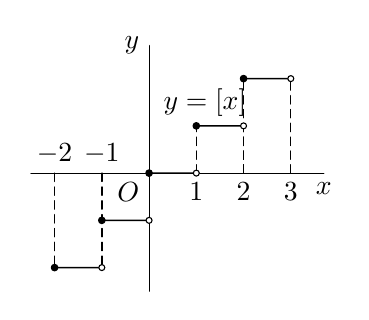
\begin{tikzpicture}[line cap=round,line join=round,scale=0.6]
        \draw[\myaxisarrow] (-2.5,0) -- (3.7,0) node[below] {$x$};
        \draw[\myaxisarrow] (0,-2.5) -- (0,2.7) node[left] {$y$};
        \foreach \i in {-2,1,2}
          {\draw[line width=0.5pt, densely dashed] (\i,0)--(\i,\i) (\i+1,0)--(\i+1,\i);}
        \foreach \i in {-2,...,2}
          {\draw[fill=black,line width=0.6pt] (\i,\i) circle (1.8pt) --(\i+1,\i);
           \draw[fill=white] (\i+1,\i) circle (1.8pt);}
        \foreach \i in {-2,-1}
          {\draw (\i,0) node[above] {$\i$};}
        \foreach \i in {1,2,3}
          {\draw (\i,0) node[below] {$\i$};}
        \draw (0,0) node[anchor=north east] {$O$} (0.1,1.5) node[right] {$y=[x]$};
      \end{tikzpicture}}
    \begin{center}
    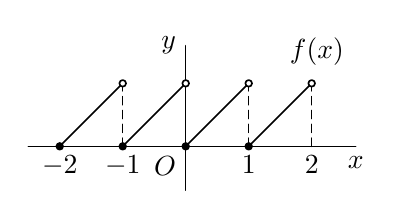
\begin{tikzpicture}[line cap=round,line join=round,scale=0.8]
      \draw[\myaxisarrow] (-2.5,0) -- (2.7,0) node[below] {$x$};
      \draw[\myaxisarrow] (0,-0.7) -- (0,1.6) node[left] {$y$};
      \foreach \i in {-1,1,2}
        {\draw[line width=0.5pt, densely dashed] (\i,0)--(\i,1);}
      \foreach \i in {-2,-1,0,1}
        {\draw[fill=black,line width=0.6pt] (\i,0) circle (1.5pt) --(\i+1,1);
         \draw[fill=white,line width=0.6pt] (\i+1,1) circle (1.5pt);}
      \foreach \i in {-2,-1,1,2}
        {\draw (\i,0) node[below] {$\i$};}
      \draw (0,0) node[anchor=north east] {$O$} (1.5,1.5) node[right] {$f(x)$};
    \end{tikzpicture}
    \end{center}
  \endsolution
  
  \lianxi
  \begin{exercise}[s]
    设函数 $D(x)=\begin{cases}
      1, & x\text{ 为有理数,}\\
      0, & x\text{ 为无理数,}\end{cases}$
    则下列结论中正确的是\,?(填序号)
    
    (1) $D(x)$ 的值域为 $\{0,1\}$;\qquad
    (2) $D(x)$ 是偶函数;
    
    (3) $D(x)$ 不是周期函数;\qquad
    (4) $D(x)$ 不是单调函数.
  \end{exercise}

  \beginsolution
    (1) 显然正确; 由 $x$ 与 $-x$ 要么同为有理数, 要么同为无理数知 $D(x)=D(-x)$, (2) 正确; 由 $D(x+1)=D(x)$ 知 (3) 错误 (任一有理数均为 $D(x)$ 的周期); 由 $D(0)=D(2)=1>0=D(\sqrt2)$ 知 (4) 正确.
  \endsolution
  
  \subsubsection{课堂评价}
  \begin{exercise}
    若函数 $f(x)=-x^2+2ax$ 与 $g(x)=\frac{a}{x+1}$ 都是 $[1,2]$ 上的单调递减函数, 则实数 $a$ 的取值范围是\,?
  \end{exercise}

  \beginsolution
    $f(x)$ 轴为 $x=a$, 开口向下, 则 $a\leqslant 1$. 由 $g(x)$ 图象知 $a>0$, 所以 $a\in(0,1]$.
  \endsolution
  
  \begin{exercise}
    若函数 $f(x)=(x+a)(x-4)$ 为偶函数, 则 $a=$\,?
    \mymarginpar{可以验证:\\
      \hbox{\quad} 多项式函数为奇函数\\
      $\Leftrightarrow$ 式中只有奇数次项;\\
      \hbox{\quad} 多项式函数为偶函数\\
      $\Leftrightarrow$ 式中只有偶数次项.}
  \end{exercise}

  \beginsolution
    $f(-x)=f(x)$, 则 $a=4$.
  \endsolution
  
  \begin{exercise}
    下列函数中, 既是偶函数又在 $(0,+\infty)$ 上单调递减的是\,?
    
    (1) $y=\frac1x$;\qquad (2) $y= \mathrm{e}^{-x}$;\qquad
    (3) $y= -x^2+1$;\qquad (4) $y= \lg|x|$.
  \end{exercise}

  \beginsolution
    (1) 奇函数且在 $(0,+\infty)$ 上 $\searrow$; 
    (2) 无奇偶性且在 $(0,+\infty)$ 上 $\searrow$; 
    (3) 偶函数且在 $(0,+\infty)$ 上 $\searrow$; 
    (4) 偶函数且在 $(0,+\infty)$ 上 $\nearrow$.
  \endsolution

  \begin{exercise}
    若函数 $f(x)= \frac1{2^x-1}+a$ 为奇函数, 则 $a=$\,?
  \end{exercise}

  \beginsolution
    $f(-x)+f(x)=0$, 则 $a=\frac12$.
    \mymarginpar{题中 $f(x)$ 的定义域中无 $0$, 故不能用 $f(0)=0$ 来求解.}
  \endsolution
  
  \subsection{课后练习}  

  \begin{exercise}
    函数 $f(x)=|x^2-1|$ 的单调递减区间是\,?
  \end{exercise}

  \beginsolution
    作图知, 单调递减区间是 $(-\infty,-1]$ 和 $[0,1]$.
    \mymarginpar{不能答 ``单调递减区间是 $(-\infty,-1]\cup [0,1]$''.}
    \begin{center}
    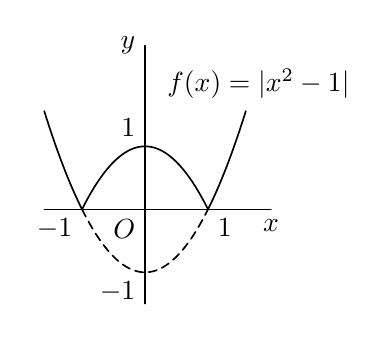
\begin{tikzpicture}[line cap=round,line join=round,scale=0.8]
      \draw[\myaxisarrow] (-1.6,0) -- (2,0) node[below] {$x$};
      \draw[\myaxisarrow] (0,-1.5) -- (0,2.6) node[left] {$y$};
      \draw[line width=0.6pt,smooth,samples=100] plot[domain=-1.6:-1](\x,{(\x)^2-1}) plot[domain=-1:1](\x,{1-(\x)^2}) plot[domain=1:1.6](\x,{(\x)^2-1});
      \draw[line width=0.6pt,smooth,samples=100, densely dashed] plot[domain=-1:1](\x,{(\x)^2-1});
      \draw (-1,0) node[anchor=north east] {$-1$}
        (0,0) node[anchor=north east] {$O$}
        (1,0) node[anchor=north west] {$1$}
        (0,-1) node[anchor=north east] {$-1$}
        (0,1) node[anchor=south east] {$1$}
        (0.2,2) node[right] {$f(x)=|x^2-1|$};
    \end{tikzpicture}
    \end{center}
  \endsolution
  
  \begin{exercise}
    定义域为 $\mathbb{R}$ 的四个函数 $y=x^3$, $y=2^x$, $y=x^2+1$, 
    $y=2\sin x$ 中, 奇函数的个数是\,?
  \end{exercise}

  \beginsolution
    $y=x^3$, $y=2\sin x$ 为奇函数, 共两个.
  \endsolution
  
  \begin{exercise}
    已知函数 $f(x)=ax^2 +4(1-a)x+1$ 在 $[1,+\infty )$ 上是单调递增函数,
    那么实数 $a$ 的取值范围是\,?
  \end{exercise}

  \beginsolution
    若 $a=0$, 则 $f(x)=4x+1$ 为单调递增函数. 若 $a\neq 0$, 则 $a>0$ 且 $-\frac{4(1-a)}{2a}\geqslant 1$, 解得 $a\geqslant 2$. 综上可知, $a\in \{0\}\cup [2,+\infty)$.
  \endsolution
  
  \begin{exercise}
    已知定义在 $\mathbb{R}$ 上的函数 $f(x)$ 对任意 $m\neq n$, 
    总有 $\frac{f(m)-f(n)}{m-n}>0$. 
    若 $f(-3)=a$, $f(-1)=b$, 求 $f(x)$ 在 $[-3,-1]$ 上的最大值
    (用 $a$, $b$ 表示).
  \end{exercise}

  \beginsolution
    题意表明 $f(x)\nearrow$, 所以 $f_{\max}= f(-1)=b$.
  \endsolution
    
  \begin{exercise}
    下列函数满足 ``$\forall\,x_1$, $x_2\in (0,+\infty)$, 
    $(x_1- x_2)\big(f(x_1)-f(x_2)\big)<0$'' 的有\,?(填序号)
    
    (1) $f(x)= \frac1x$; (2) $g(x)=(x-1)^2$; (3) $h(x)= \ln(x+1)$.
  \end{exercise}

  \beginsolution
    题意表明 $f(x)$ 在 $(0,+\infty) \searrow$, 故只有 $f(x)$ 符合题意.
  \endsolution

  \begin{exercise}
    设函数 $f(x)= a\sin x+x^2$, 若 $f(1)=0$, 则 $f(-1)$ 的值为\,?
  \end{exercise}

  \beginsolution
    因为 $y=\sin x$ 为奇函数, 所以
    \[f(1)=a\sin1+1,\quad (-1)=-a\sin1+1,\]
    相加得 $f(1)+f(-1)=2$, 则 $f(-1)=2$.
    
    \varexercise 设函数 $f(x)= a\sin x+b\tan x+x^2$, 若 $f(1)=0$, 则 $f(-1)$ 的值为\,?
    
    同上方法可知 $f(-1)=1$.
    
    \varexercise 设函数 $f(x)= \frac{a\sin x}{\mathrm{e}^x+\mathrm{e}^{-x}}+x^2$, 若 $f(1)=0$, 则 $f(-1)$ 的值为\,?
    
    仍然可得 $f(-1)=1$.
  \endsolution
  
  \begin{exercise}
    一次函数 $f(x)=ax+b$ 在 $[-1,1]$ 上恒正的充要条件是什么\,?
  \end{exercise}

  \beginsolution
    $f(-1)>0$ 且 $f(1)>0$, 即 $-a+b>0$ 且 $a+b>0$.
  \endsolution

  \begin{exercise}
    若函数 $f(x)=kx^2+(k-1)x+2$ 是偶函数, 求 $f(x)$ 的单调递减区间.
  \end{exercise}

  \beginsolution
    由题 $k=1$, $f(x)=x^2+2$, 则 $f(x)$ 的单调递减区间是 $(-\infty,0]$.
  \endsolution
  
  \begin{exercise}
    已知函数 $f(x)$ 为偶函数, 且当 $x<0$ 时, $f(x)=x^2 -\frac1x$,
    求 $f(1)$.
  \end{exercise}

  \beginsolution
    $f(1)=f(-1)=2$.
  \endsolution
  
  \begin{exercise}
    已知偶函数 $f(x)$ 在区间 $[0,+\infty )$ 上单调递增. 
    若 $f(2x-1)<f\Big(\frac13\Big)$, 则 $x$ 的取值范围是\,?
  \end{exercise}

  \beginsolution
    $f(|2x-1|)=f(2x-1)<f\Big(\frac13\Big)$, 则 $|2x-1|<\frac13$,  $x\in\Big(\frac13,\frac23\Big)$.
    
    \varexercise 若 $f(x)$ 改为奇函数, 其余条件不变, 则 $x$ 的取值范围是\,?
    
    此时 $f(x)$ 在 $\mathbb{R}$ 上 $\nearrow$, 则 $2x-1< \frac13$ 即 $x\in\Bigl(-\infty,\frac23\Bigr)$.
  \endsolution

%%%%%%%%%%%%%%%%%%%%%%%%%%%